\section*{Fra Rådhuset til Munchmuseet}

I matematikk liker man å vri å vende på konsepter man kanskje kjenner til allerede, for eksempel avstand. De fleste av oss har lært om Pytagoras’ læresetning i løpet av grunnskolen, som sier at $a^2+b^2=c^2$ for en rettvinklet trekant med kateter $a$ og $b$, og hypotenus $c$. Siden katetene står vinkelrett på hverandre kan vi se for oss at disse måler avstand i to unlike retninger.

Avstanden til punktet gitt av disse to katetene, er altså $c$, og vi kan finne denne avstanden ved å ta kvadratroten på begge sider av Pytagoras ligningen, altså 

$$
c = \sqrt{a^2+b^2}.
$$

Dette kan også skrives som $c = (a^2+b^2)^{\frac{1}{2}}$. For en matematiker ser dette veldig fristende ut å endre, ettersom vi kunne tenke oss å bytte ut tallet $2$ i ligningen med et hvilket som helst annet tall, for eksempel $(a^7+b^7)^{\frac{1}{7}}$ . For å sørge for at vi måler kun ‘positiv avstand’ tar vi absoluttverdien av $a$ og $b$ inne i dette utrykket. Dette kalles å måle avstand med $7$-norm, og i det generelle tilfellet $(|a|^p+|b|^p)^{\frac{1}{p}}$ kaller vi å måle avstand med $p$-norm. En litt mer vanlig måte å beskrive dette på er å ta en vektor $\vec x = (x_1, x_2)$ og skrive

$$
\Vert \vec x \Vert_p = (|x_1|^p+|x_2|^p)^{\frac{1}{p}} = \left(\sum_{i=1}^2 |x_i|^p\right)^{\frac{1}{p}}.
$$

Vi kan da se at måten vi måler avstand med til hverdags er bare et eksempel av alle disse måtene vi kunne ha gjort det på, det er nemlig $p$-normen med $p=2$. 

Kanskje tenker du at de andre måtene å måle avstand på bare er helt tullete — hvorfor skal vi bry oss om dette? Se for deg at du står midt i Manhattan i New York. Gatesystemet er et rutenett med to ulike retninger, og du vil bevege deg fra en side av et kvartal til motsatt side, altså rundt på baksiden. 

\begin{center}
    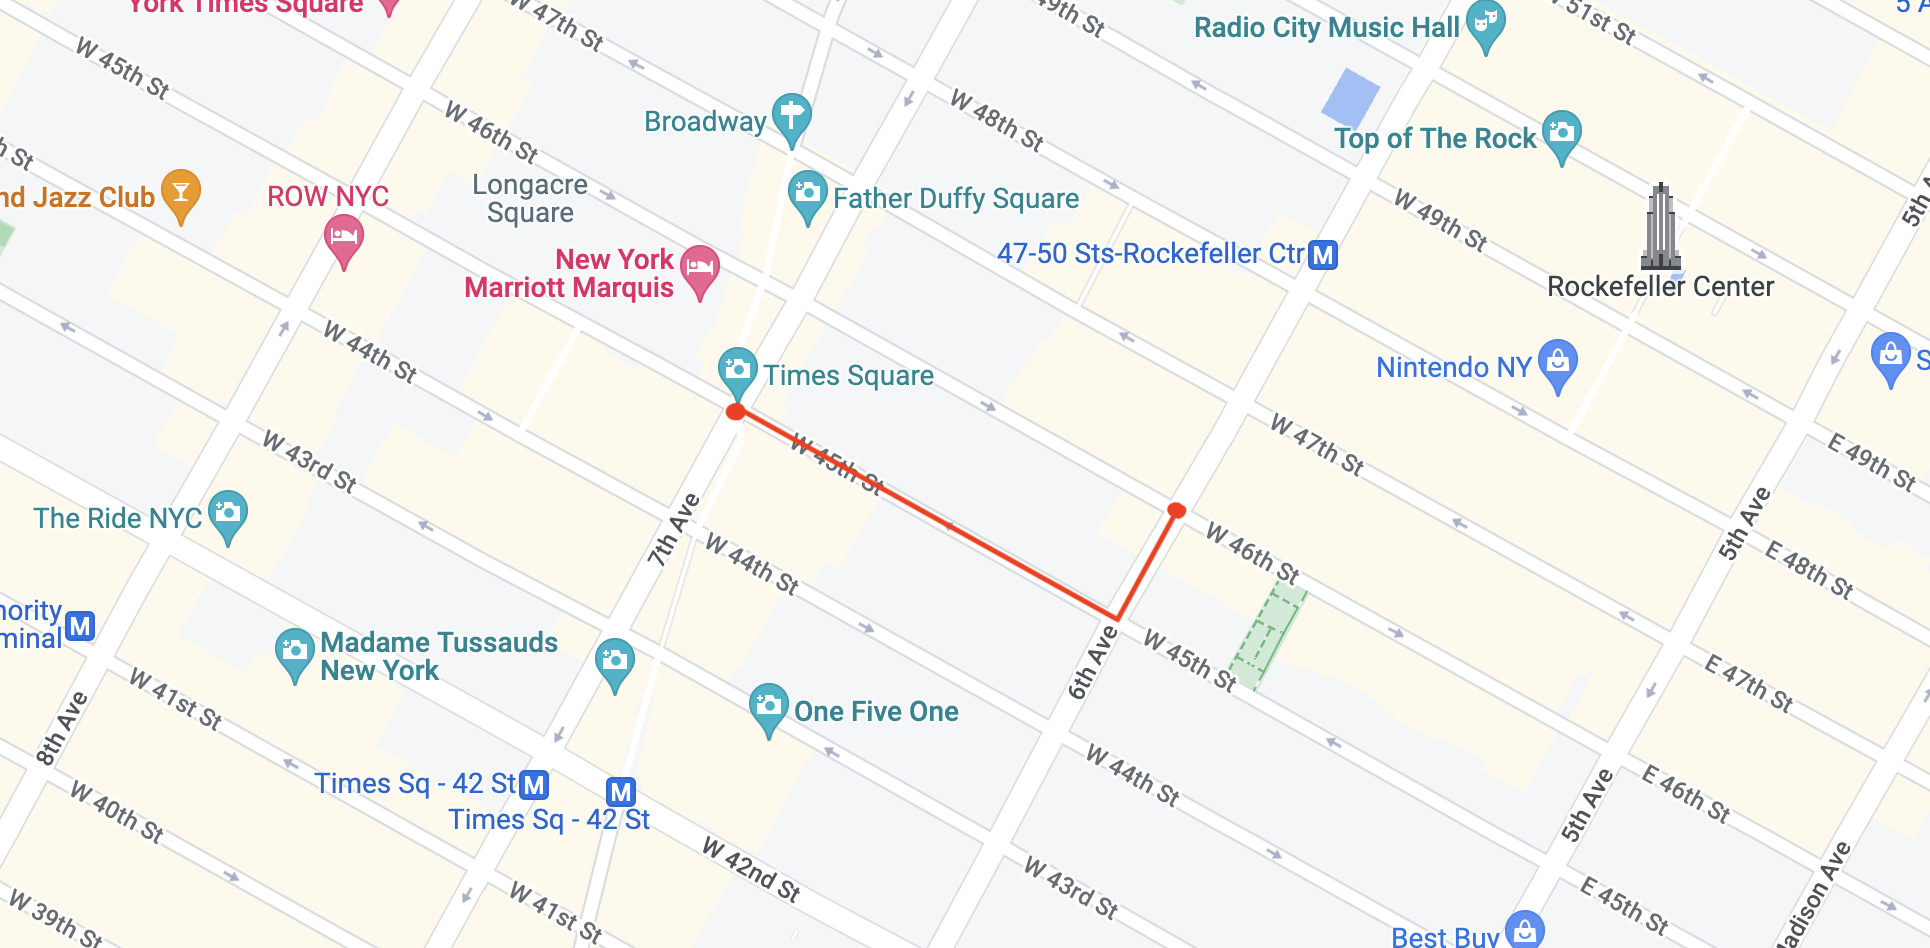
\includegraphics[width=\textwidth]{img/manhattan.png}
\end{center}

Måler vi avstand med den vanlige metoden får vi en rett linje som går diagonalt gjennom kvartalet, noe som ikke forteller oss hvor langt det faktisk er å gå, ettersom vi kun gan gå rundt. Dermed må vi måle avstand litt annerledes. Måten å gjøre dette på i Manhattan er å måle først strekningen i den ene retningen, og så plusse på strekningen i den andre retningen. Dette er nøyaktig det samme som å måle avstand med $1$-normen! Grunnet dette kalles $1$-normen ofte Taxi-normen, ettersom den beskriver hvor langt en taxi må kjøre i Manhattan for å komme seg til et sted. 

På den andre enden av spekteret har vi grenseverdien når $p\to \infty$. Denne normen kan også beskrives ved 

$$
\Vert \vec x \Vert_\infty = \max\{|x_1|, |x_2|\}.
$$

Nå har vi alt vi trenger for å løse oppgaven. Vi har oppgitt at vi befinner oss i $(0,0)$ og at destinasjonen vår er på land mot øst med $1$-norm avstand $\Vert \vec x \Vert_1 = |x_1|+|x_2| = 1.9\mathrm{km}$ og $\infty$-norm avstand $\Vert \vec x \Vert_\infty = \max\{|x_1|, |x_2|\}=1.25\mathrm{km}$. Dermed vet vi automatisk at enten $|x_1|=1.25$ eller $|x_2|=1.25$, noe som betyr at den andre må være $1.9-1.25 = 0.65$. Disse kan vi enkelt legge inn på et kart og se hvor vi ender opp. 

\begin{center}
    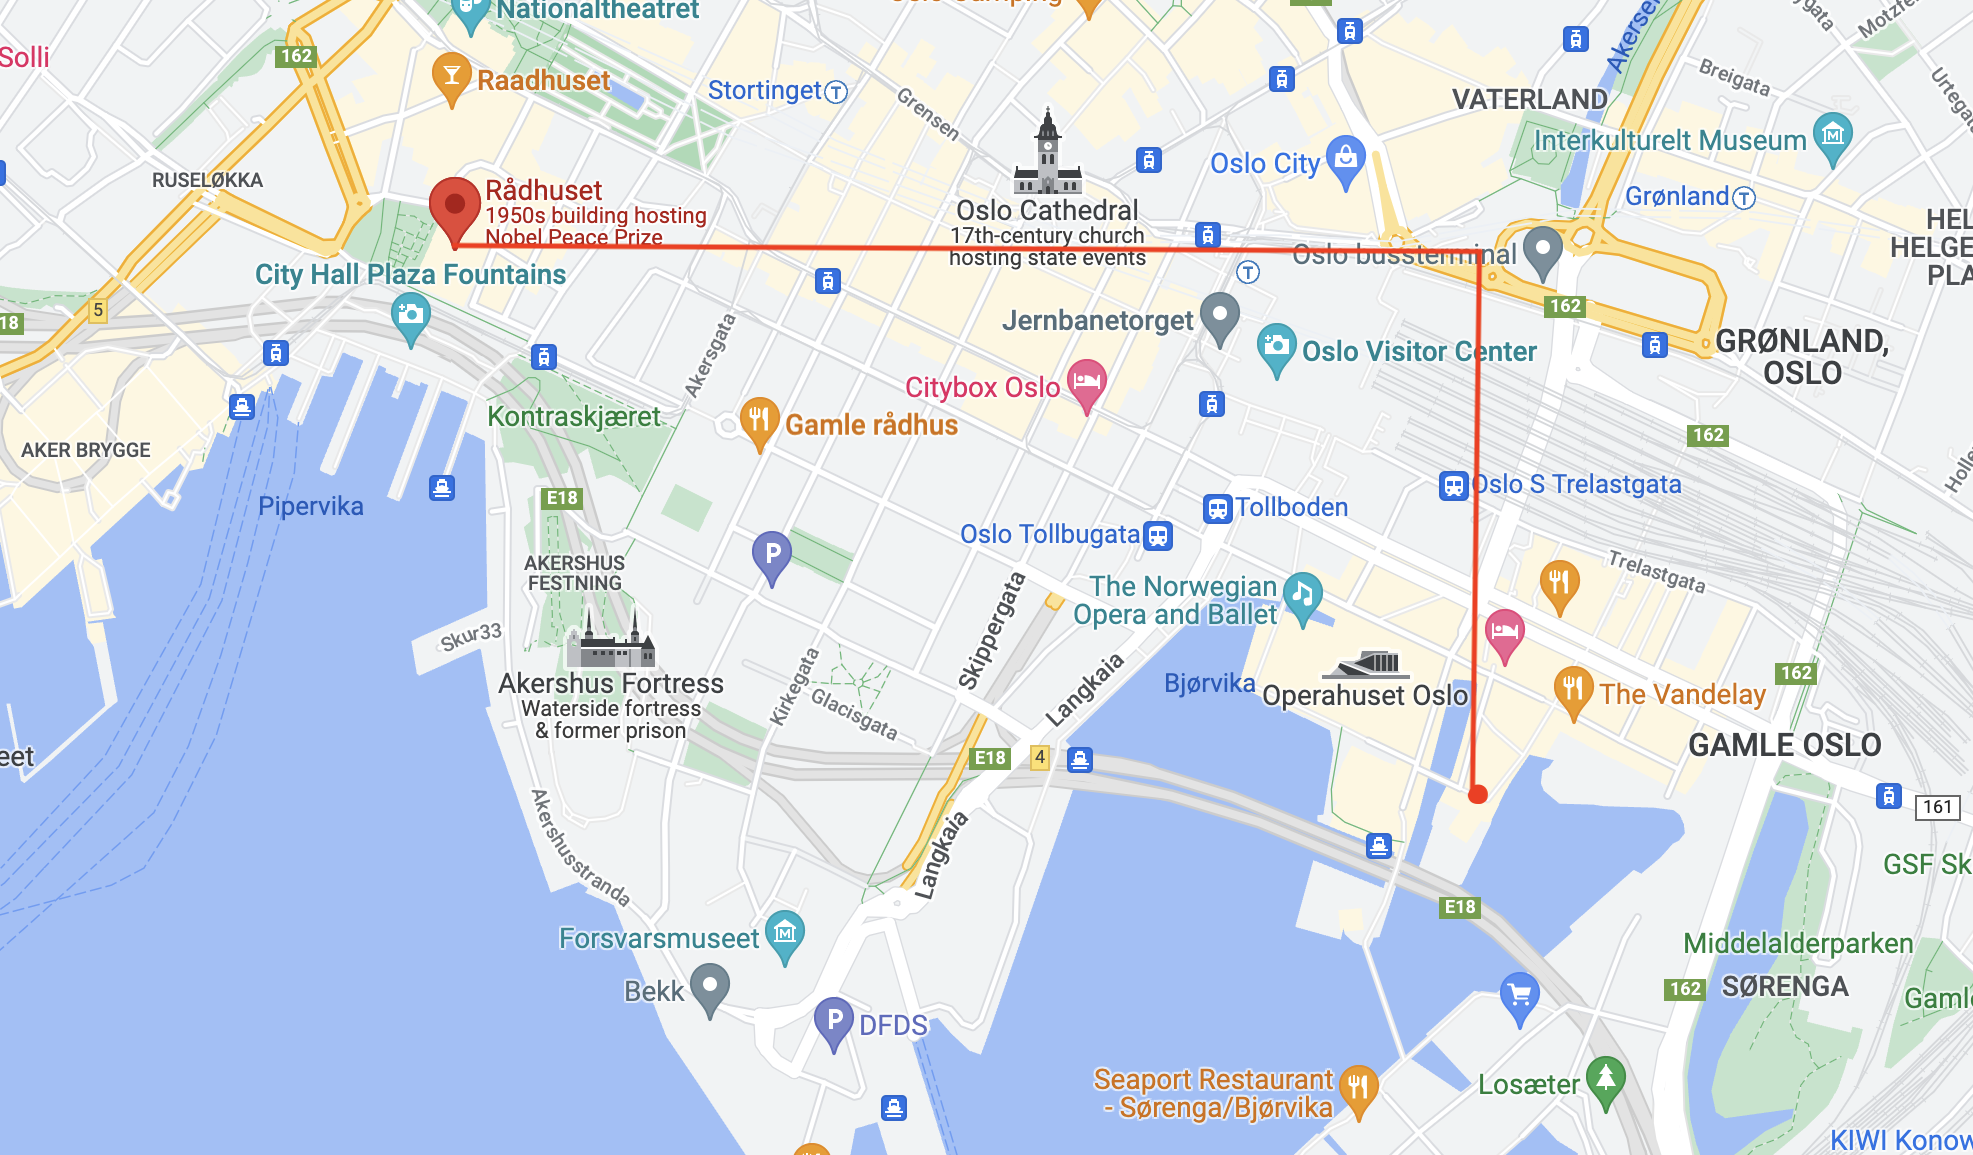
\includegraphics[width=\textwidth]{img/munch_2.png}
\end{center}

Vi ser at kun det ene punktet er på land, som betyr at det er dit vi skal. Ser vi på kartet er det nøyaktig Munch museet som er destinasjonen. 

